\section{Evaluation}

We evaluate Meerkat.Graph on single source context-free path querying scenario.
For evaluation we use Neo4j graph databese which was run on PC with the folloeing configuration.
\begin{itemize}
  \item CPU
  \item RAM
  \item OS
  \item JVM
\end{itemize}

Neo4j is integreted into application !!!!

Dataset contains two real-world RDFs: Geospecies which contains information about biological hierrarchy\footnote{\url{https://old.datahub.io/dataset/geospecies}. Access date: 12.11.2019.} and Enzime which is a part of UniProt database\footnote{Protein sequences data base: \url{https://www.uniprot.org/}. RDFs with data are avalable here: \url{ftp://ftp.uniprot.org/pub/databases/uniprot/current_release/rdf}. Access date: 12.11.2019}.
Detailed description of these graphs is presented in table~\ref{tbl:datasetDetails}.
Note, that graphs was loaded into database fully, not only edges which laballed by relations used inqueryes.

\begin{table}[ht]
\begin{tabular}{|c|c|c|c|c|c|}
\hline
 Graph & \#Vertices & \#Edges & \#NT & \#BT \\
 \hline
 Enzime &  &  &  &  \\
 Geospecies &  &  &  &  \\
 \hline
\end{tabular}
\caption{Details of graphs}
\label{tbl:datasetDetails}
\end{table}

Queries for evaluation are versions of same-generation query --- classical context-free query which is useful for hierarchy analysis.
We equip queryes with user-defined actions for end verties saving, paths length calcualtion and unique path counting.
To demonstarte power of combinators, we use the function !!! defied above to create queries.

For each graph and each query we run this query form each vertex from graph and measure elapsed time and required memory by using !!! tool.
Note, that mesured memory is allocated by JVM, not really used.


\textbf{Enzime RDF querying.} We evaluate two queryes: $Q_1$ --- same genaration over !!!! relation
\begin{lstlisting}
def sameGen(brs) =
  reduceChoice(
    brs.map {case (lbr, rbr) =>
      lbr ~ syn(sameGen(brs).?) ~ rbr})
\end{lstlisting}

and $Q_2$ --- same generation over !!!
\begin{lstlisting}
def sameGen(brs) =
  reduceChoice(
    brs.map {case (lbr, rbr) =>
      lbr ~ syn(sameGen(brs).?) ~ rbr})
\end{lstlisting}
.

Results of evaluation are presented in figures~\ref{fig:enzime_time_per_paths} and~\ref{fig:enzime_mem_per_paths}.
Also we collect paths length destribution which is showed in figure~\ref{fig:pLength}.
We can see that prvided datasets contain relatively short paths which satisfie queryes.


\begin{figure}
\centering
  \subcaptionbox{Enzime\label{fig:pLengthEnzime}}
    {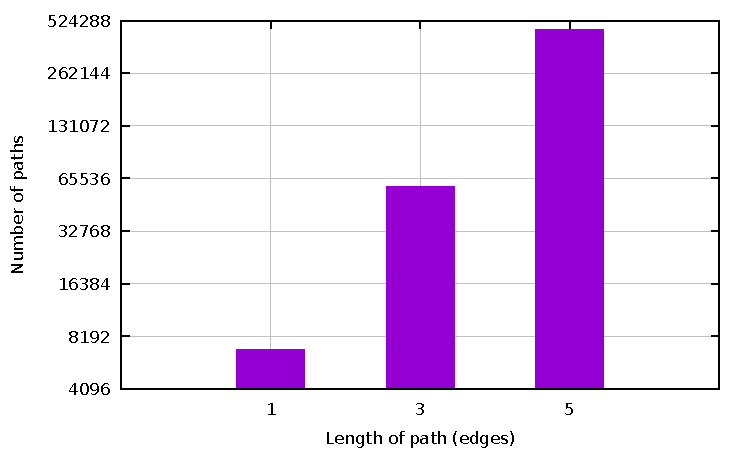
\includegraphics[width=0.23\textwidth]{data/enzime_narrowerTr_path_per_length.pdf}}
\subcaptionbox{Geospecies\label{fig:pLengthGeospecies}}
{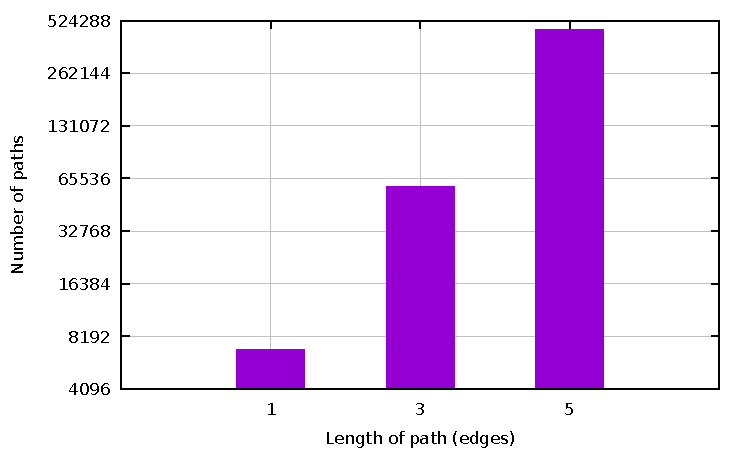
\includegraphics[width=0.23\textwidth]{data/enzime_narrowerTr_path_per_length.pdf}}
\caption{Paths length destribution}\label{fig:pLength}
\end{figure}

\begin{figure}[ht]
  \begin{center}
    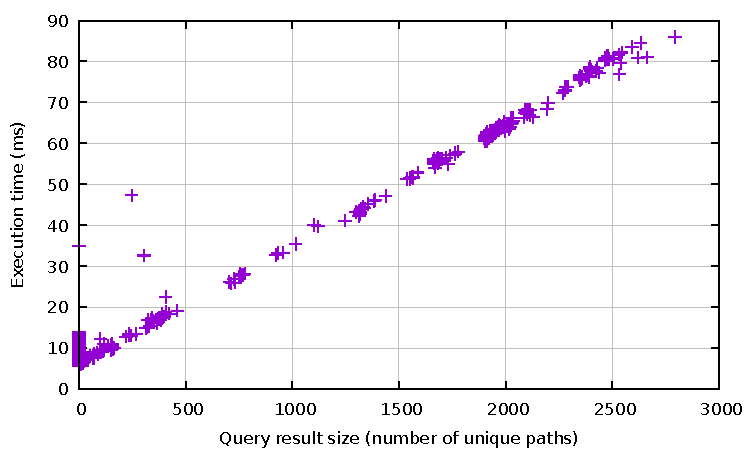
\includegraphics[width=0.5\textwidth]{data/enzime_narrowerTr_time_per_paths.pdf}
    \caption{Query execution time for Enzime dataset and queryes $Q_1$ and $Q_2$}
    \label{fig:enzime_time_per_paths}
  \end{center}
\end{figure}

Figure~\ref{fig:enzime_time_per_paths} shows dependency of query evaluation time on query answer size in terms of number of edge-different !!! paths.
First of all, we can see that evaluation time is linear on answer size.
Also we can see, that time which requred to evaluate query for one specific vertex is relatively small.
In our case it is less than 90ms.

\begin{figure}[ht]
  \begin{center}
    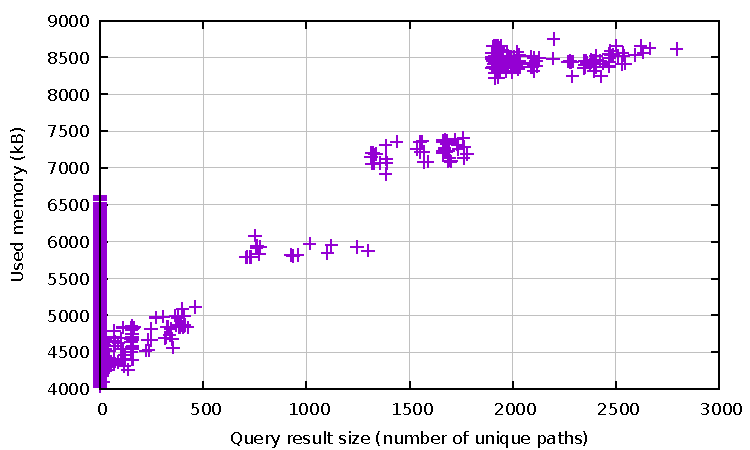
\includegraphics[width=0.5\textwidth]{data/enzime_narrowerTr_mem_per_paths.pdf}
    \caption{Query required memory for Enzime dataset and queryes $Q_1$ and $Q_2$}
    \label{fig:enzime_mem_per_paths}
  \end{center}
\end{figure}

Figure~\ref{fig:enzime_mem_per_paths} shows dependency of memory requred to evaluate qurey on query answer size in terms of number of uniqie paths.


\textbf{Geospecies RDF querying.}

\begin{figure}[ht]
  \begin{center}
    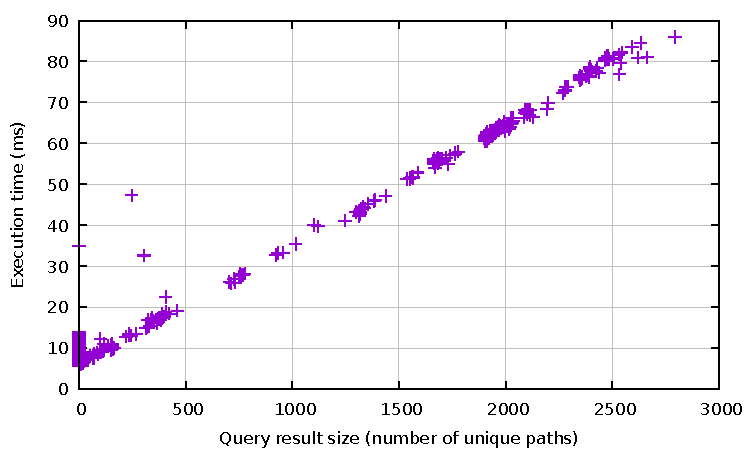
\includegraphics[width=0.5\textwidth]{data/enzime_narrowerTr_time_per_paths.pdf}
    \caption{Query execution time for Enzime dataset and queryes $Q_3$ and $Q_4$}
    \label{fig:geo_time_per_paths}
  \end{center}
\end{figure}

Here we can see !!!!

\begin{figure}[ht]
  \begin{center}
    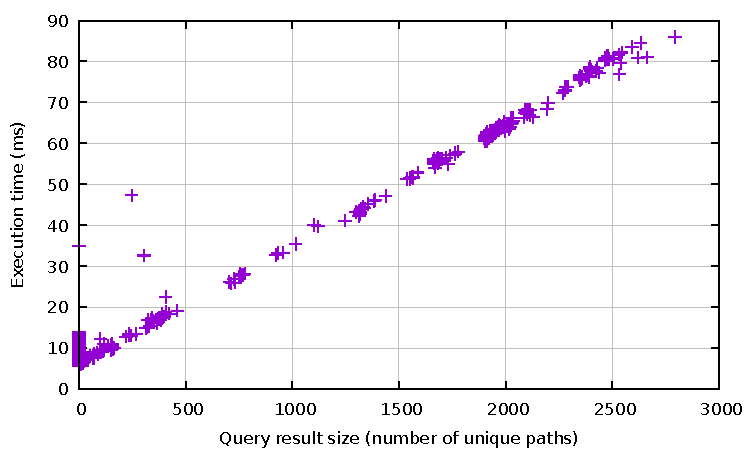
\includegraphics[width=0.5\textwidth]{data/enzime_narrowerTr_time_per_paths.pdf}
    \caption{Query execution time for Enzime dataset and queryes $Q_3$ and $Q_4$}
    \label{fig:geo_time_per_paths}
  \end{center}
\end{figure}

Finally, we can conclude that confext-free path querying in single source scenario can be efficiently evaluated by using !!! in case when number of paths in answer is big but its length is relatively small. While all pairs scenario is still hard ~\cite{!!!}, single source scenarion, which is useful for manual or interactive data analysis, can be !!!
